\documentclass[a4paper, 10pt]{article}
\usepackage[italian]{babel}
\usepackage{amsmath, amsfonts, amssymb, amsthm}
\usepackage{graphicx}
\usepackage{hyperref}

\begin{document}
\title{\textbf{Alberi di decisione con dati mancanti}}\date{}
\author{Athos Innocenti}
\maketitle
\section{Introduzione}
Lo scopo di questo elaborato è di implementare l'algoritmo di apprendimento per \textbf{alberi di decisione} con l'aggiunta di una strategia per la gestione di \textbf{dati mancanti}.

Questa strategia consiste nell'assegnare una probabilità a ciascun possibile valore di un attributo in base all'insieme di esempi disponibili in un certo nodo dell'albero (una tecnica dunque più complessa rispetto a quella in cui si assegna al dato mancante il valore più comune dell'attributo in un certo insieme di esempi).

La probabilità viene stimata in base alle frequenze osservate dei singoli valori dell'attributo tra gli esempi noti all'interno di un certo nodo dell'albero di decisione. Una volta definita la probabilità per ciascuno dei possibili valori, una frazione dell'esempio con il dato mancante viene distribuita per ciascuno dei valori possibili nei corrispettivi sotto-alberi.

Questi esempi vengono utilizzati per il calcolo del \textit{gain} e possono essere ulteriormente divisi in altri sotto-alberi se deve essere testato il valore mancante di un altro attributo. 
\section{Base teorica}
In un albero di decisione i \textbf{nodi} interni, inclusa la radice, rappresentano dei \textbf{test} sugli attributi. I figli di un nodo, limitandosi al caso di attributi categorici, sono tanti quanti i possibili valori che l'attributo nel nodo padre può assumere e ciascuno di essi conterrà un altro attributo, cioè un nuovo test.

Il valore della funzione definita dall'albero di decisione viene letto nella foglia raggiunta seguendo un cammino nell'albero in relazione alle risposte date ai test nei nodi incontrati. 

Il \textbf{bias induttivo} che sta alla base dell'algoritmo per la costruzione degli alberi di decisione è che tra tutti i possibili alberi si vuole prendere l'albero più piccolo che faccia un buon fit dei dati.

L'algoritmo procede trovando l'attributo che permette di fare uno split che riduca quanto più possibile l'\textbf{impurità} del dataset risultante. Questa scelta viene fatta in relazione ad una quantità detta \textbf{gain} definita rispetto all'impurità del dataset.

Indicata con $\hat{p_{k}}$ la porzione di esempi che appartengono alla classe $k$, con $K$ il numero di classi possibili, e posto $k^{*}$ la classe più frequente su un certo dataset, le possibili misure di impurità utilizzabili sono:
\begin{enumerate}
\item\textbf{Errore di classificazione}  si assegna a tutti gli esempi del dataset corrente la classificazione della classe di maggioranza $k^{*}$ e si definisce l'errore di classificazione come $1 - \hat{p_{k^*}}$.
\item\textbf{Indice di Gini} è definito come $\sum_{k=1}^{K}\hat{p_{k}}(1 - \hat{p_{k}})$ considerando quindi ogni possibile classe $k$.
\item\textbf{Entropia} è definita come numero medio di bit necessari per codificare un simbolo in una sorgente di informazione: $-\sum_{k=1}^{K}\hat{p_{k}}log_2{\hat{p_{k}}}$.
\end{enumerate}
In questo progetto è stata utilizzata l'entropia come misura di impurità.
\section{Datasets}
I datasets utilizzati nel progetto sono tutti reperibili presso il sito \textbf{UCI Machine Learning Repository} e sono i seguenti:
\begin{enumerate}
\item\textbf{Tic-Tac-toe Endgame}
\item\textbf{Monk's Problems}
\item\textbf{Balance Scale}
\end{enumerate}
Per semplicità sono stati considerati solo datasets con attributi categorici. Come già accennato nell'introduzione, per ricondursi alla gestione del problema dei dati mancanti, per ciascun valore di probabilità considerato (0, 0.1, 0.2 e 0.5), all'interno del training set vengono eliminati in modo casuale ed uniforme, con probabilità \textit{p} crescente, alcuni valori degli attributi dagli esempi.
\section{Apprendimento e overfitting}
Per la gestione della fase di apprendimento è stata utilizzata la tecnica chiamata \textbf{Grid Search Cross Validation}.

Inizialmente si estrae il $20\%$ del dataset che viene utilizzato come test set nella fase finale del progetto.

Il rimanente $80\%$ viene utilizzato per la \textit{K-Fold Cross Validation} tramite la quale viene diviso in cinque blocchi di esempi aventi la medesima dimensione (\textit{k} indica il numero di blocchi considerati). A turno, e per una volta ciascuno, ognuno dei cinque blocchi viene utilizzato come validation set mentre i rimanenti quattro blocchi vengono presi insieme per costituire il training set.

La tecnica della cross validation permette dunque di allenare il modello su ciascun segmento (anche detto blocco) evitando così problemi di overfitting sui dati. Sostanzialmente si esclude a turno un blocco cercando di predirlo utilizzando i blocchi rimanenti.

Durante ciascun turno viene applicata la \textit{Grid Search}, una tecnica di ottimizzazione degli iperparametri (in questo caso si ha un solo iperparametro rappresentato dalla profondità dell' albero) che permette di ricavare quel valore dell'iperparametro con il quale è possibile raggiungere la performance migliore. Per farlo si creano molteplici modelli, quindi molteplici alberi di decisione, ciascuno con un valore diverso dell'iperparametro e alla fine si seleziona il valore dell'iperparametro con cui si ha la performance migliore.

Applicando questa tecnica si crea inizialmente l'albero di decisione avente profondità massima, se ne calcola l'accuratezza rispetto al validation set e successivamente si vanno a costruire tutti gli alberi interrompendo la loro creazione ad una profondità crescente partendo dalla profondità minima (i.e. 1 si prende solo la radice dell'albero con i suoi figli come foglie) fino ad arrivare alla profondità massima (la profondità del primo albero costruito). Per ciascuno di questi alberi si calcola la sua accuratezza in relazione al medesimo validation set. La validazione di ciascun albero si basa sul blocco del turno corrente selezionato come validation set, mentre la costruzione di ciascun albero utilizza i rimanenti quattro blocchi.

Come passo finale di ciascun turno si determina la profondità che ha permesso di raggiungere l'accuratezza massima memorizzandola in una lista.

Una volta conclusi tutti i turni, quindi dopo che ciascuno blocco è stato utilizzato una volta come validation set, si calcola la moda delle profondità ricavate e si costruisce l'albero di decisione utilizzando come training set tutti e cinque i blocchi limitando la sua costruzione alla profondità corrispondente alle moda appena calcolata.

Dato quindi l'albero di decisione finale, si calcola la sua accuratezza in relazione al test set inizialmente costruito.

Questa tecnica viene quindi ripetuta per ogni valore di probabilità considerato e permette di gestire il problema dell'\textit{overfitting}. Il test set è sempre il medesimo per tutti i valori di probabilità.
\section{Implementazione ed Esecuzione}
Il progetto è stato realizzato utilizzando \textit{Python 3.8} e alcune librerie esterne riportate nel \textbf{README} per il calcolo scientifico e per visualizzare i risultati mediante l'ausilio di grafici. L'intera esecuzione del codice viene gestita nel \textbf{main}. Il primo passo è quello di caricare il dataset invocando i metodi \textit{get attributes} e \textit{get examples} della classe \textbf{dataset} per ottenere gli attributi del dataset e tutti gli esempi che lo compongono insieme al vettore delle classificazioni. Si procede definendo gli indici per ciascun attributo ed esempio, si estrapolano i valori degli attributi e della classe tramite \textit{get attributes values} e \textit{get target values}. Dopo aver estratto il $20\%$ degli esempi che costituiranno il test set, per ciascun valore della probabilità considerato viene applicata la \textbf{grid search cross validation} durante la quale verranno costruiti i vari alberi di decisione tramite il metodo \textit{dt learning} della classe \textbf{DecisionTree} utilizzando il rimanente $80\%$ del dataset suddiviso come già descritto sopra. Come ultima operazione viene plottato il grafico dell'accuratezza dell'albero di decisione finale costruito per ciascun valore della probabilità \textit{p} e valutato rispetto al test set.
\section{Risultati}
In riferimento ai grafici riportarti qui di seguito, relativi ai tre datasets utilizzati, è possibile osservare come l'accuratezza sul test set dell'albero di decisione tende a diminuire all'aumentare della probabilità \textit{p} di eliminare dei valori degli attributi nel training set (nei tre grafici l'accuratezza è riportata in \textit{percentuale}).
\newpage
\begin{figure}[h]
\centering
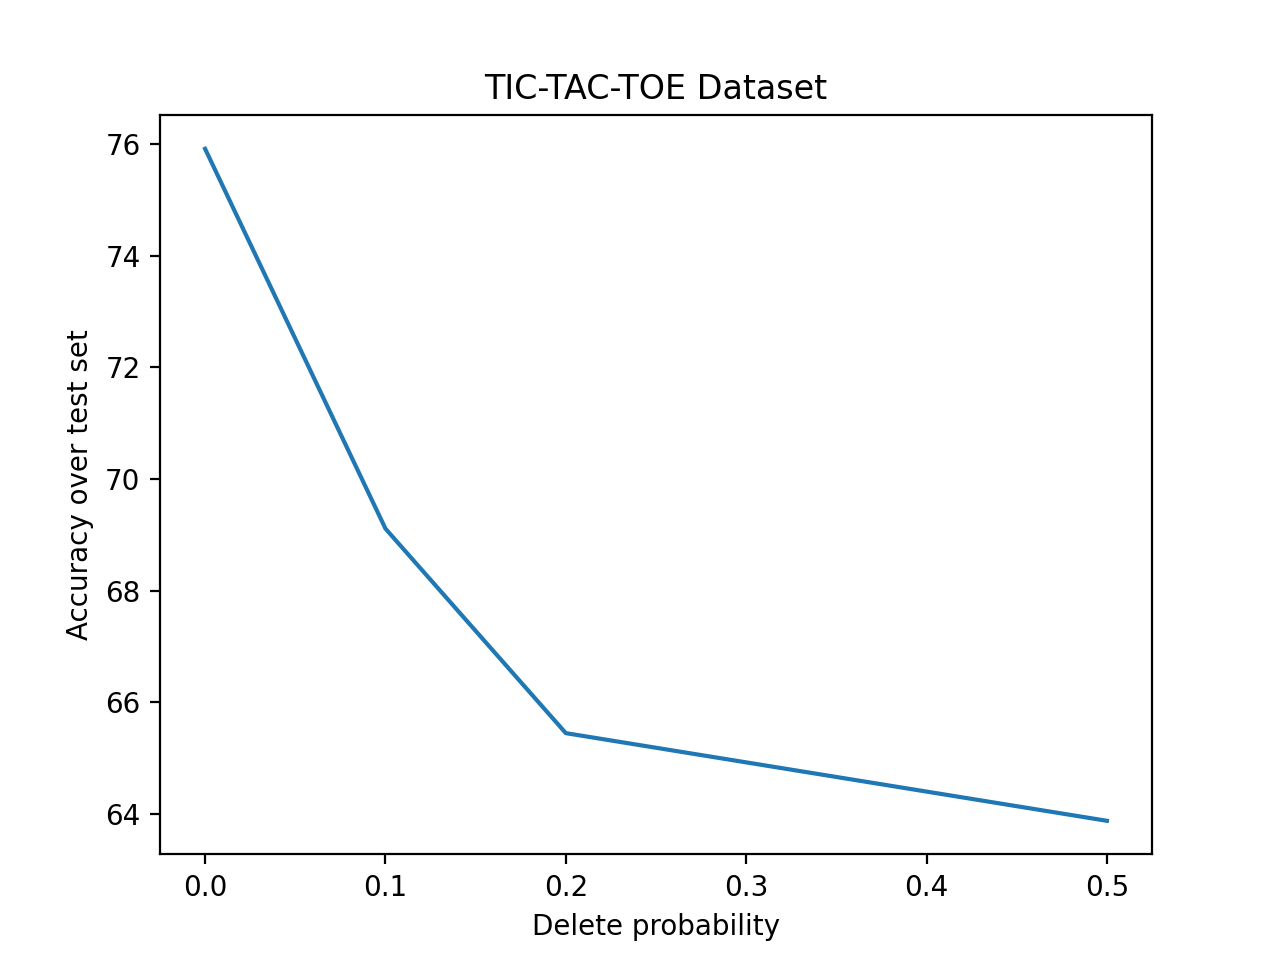
\includegraphics[scale=0.3,angle=0]{tic_tac_toe.png}
\caption{Andamento dell'accuratezza per il dataset \textbf{Tic-Tac-Toe}}
\end{figure}
\begin{figure}[h]
\centering
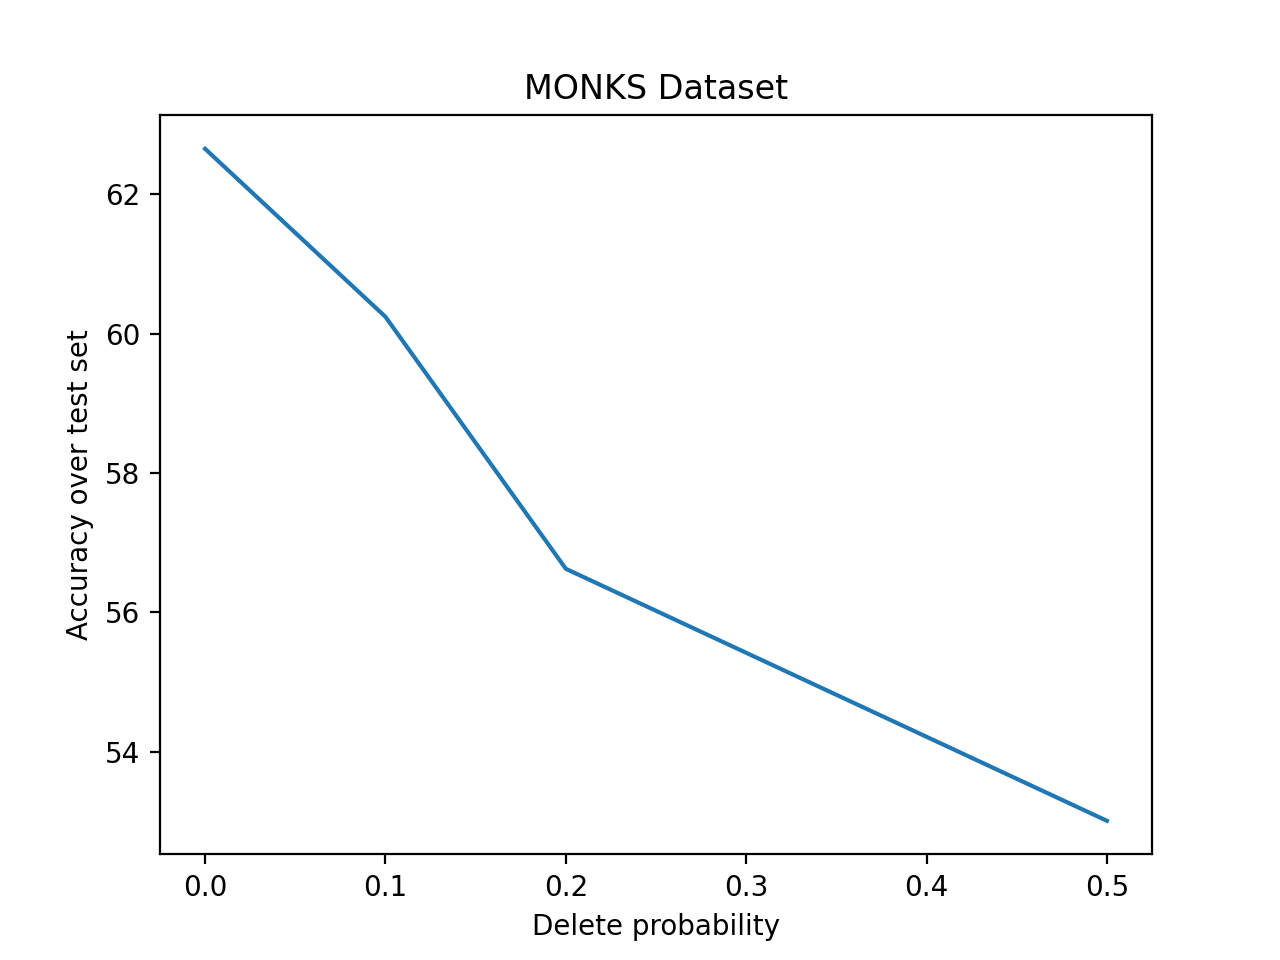
\includegraphics[scale=0.3,angle=0]{monks.png}
\caption{Andamento dell'accuratezza per il dataset \textbf{Monk's Problems}}
\end{figure}
\begin{figure}[h]
\centering
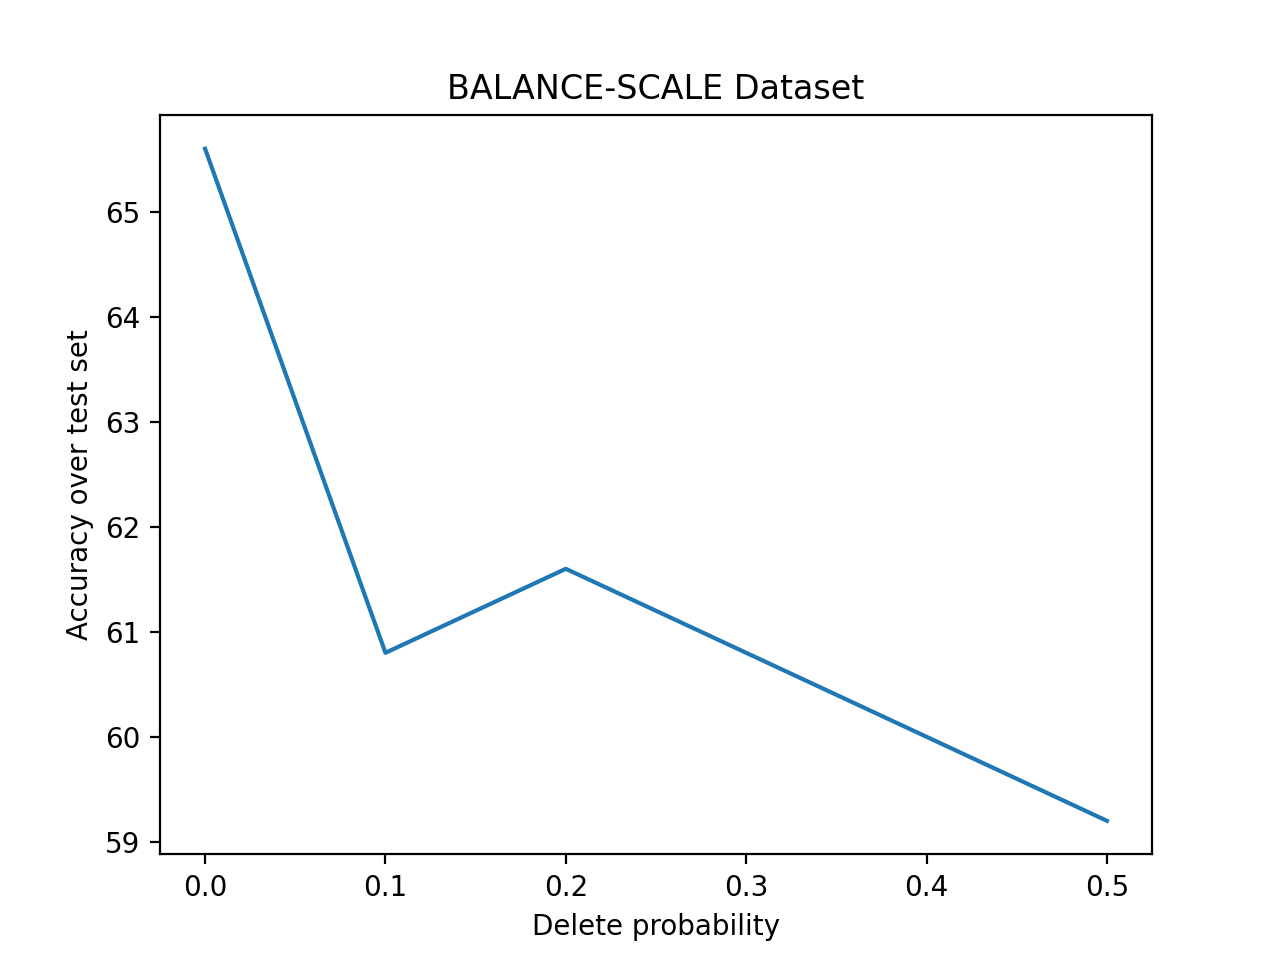
\includegraphics[scale=0.3,angle=0]{balance_scale.png}
\caption{Andamento dell'accuratezza per il dataset \textbf{Balance Scale}}
\end{figure}
\section{Fonti}
\begin{enumerate}
\item[]S. Russell P. Norvig. \textit{Artificial Intelligence A Modern Approach} 3rd Edition, Pearson, 2010
\item[]Mitchell. \textit{Decision Tree Learning}, 1997
\end{enumerate}
\end{document}